\documentclass{beamer}
\mode<presentation>{\usetheme{Custom}}

\usepackage[orientation=portrait,size=a0,scale=1.4,debug]{beamerposter}
\usepackage[french]{babel}
\usepackage[utf8]{inputenc}
\usepackage{graphicx}
\usepackage{xcolor}
\usepackage{tcolorbox}
\usepackage{tikz}


\tikzset{every picture/.style={execute at begin picture={
   \shorthandoff{:;!?};}
}}

\tikzset{rndblock/.style={rounded corners,rectangle,draw,outer sep=0pt}}
\newcommand{\tframed}[2][]{\tikz[baseline=0.1pt]\vspace{0.1cm}\node[rndblock,minimum height=1.5em,#1] (m) {#2} ;}
\newcommand{\hilight}[1]{\textbf{\tframed[blue,fill=blue!10]{#1}}}
\newcommand{\whilight}[1]{\textbf{\tframed[purple,fill=purple!10]{#1}}}


\newcommand{\sP}{\hspace{1pt}}
\newcommand{\mP}{\hspace{3pt}}
\newcommand{\bP}{\hspace{6pt}}
\newcommand{\BP}{\hspace{12pt}}

\definecolor{OrangeRed}{RGB}{255, 40, 0}
\definecolor{darksalmon}{RGB}{233,150,122}
\definecolor{blendedblue}{rgb}{0.137,0.466,0.741}
\definecolor{blendedgray}{rgb}{0.838,0.833,0.833}
\definecolor{blendedpurple}{RGB}{75,20,130}
\definecolor{tgray}{rgb}{0.211, 0.211,0.244}
\definecolor{darkgray}{rgb}{0.450,0.450,0.450}
\definecolor{maroon}{rgb}{0.665, 0.142, 0.142}
\definecolor{ngreen}{rgb}{0.000,0.500,0.000}
\definecolor{dgreen}{RGB}{0,150, 0}

%%%%%%%%%%%%%%%%%%%%%%%%%%%%%%%%%%%%%%%%%%%%%%%%%%%%%%%%%%%%%%%%%%%%%%%%%%%%%%%%%%%%%%

\title{Combinaison de mots et de syllabes pour transcrire la parole}
\author{Luiza Orosanu\\\vskip1.2ex Denis Jouvet}
\institute{Équipe PAROLE, Loria\\\vskip1.2ex Nancy, France}
\date[24 Juin 2014]{24 Juin 2014}

%%%%%%%%%%%%%%%%%%%%%%%%%%%%%%%%%%%%%%%%%%%%%%%%%%%%%%%%%%%%%%%%%%%%%%%%%%%%%%%%%%%%%%
\newlength{\columnheight}
\setlength{\columnheight}{105cm}


%%%%%%%%%%%%%%%%%%%%%%%%%%%%%%%%%%%%%%%%%%%%%%%%%%%%%%%%%%%%%%%%%%%%%%%%%%%%%%%%%%%%%%
\begin{document}
\begin{frame}
\begin{columns}

% ---------------------------------------------------------%
% Set up a column
% ---------------------------------------------------------%

\begin{column}{.53\textwidth}
\begin{beamercolorbox}[center,wd=\textwidth]{postercolumn}
\begin{minipage}[T]{.98\textwidth}

\parbox[t][\columnheight]{\textwidth}
{
	\vskip-2ex
	\begin{block}{Introduction}
		\begin{itemize}
			\item {\bf \color{OrangeRed} Objectif global du projet}
				\begin{itemize}
				\item créer un dispositif portable et autonome
				\item intègrer un système de reconnaissance de la parole
					\begin{list}{\color{black!75} $\ast$}{\leftmargin=8mm \itemindent=0em}
					\vskip0.4ex
					\item l'adapter aux besoins des personnes sourdes ou malentendantes
						\begin{list}{\color{black!75}-}{\leftmargin=12mm \itemindent=0em}
						\item améliorer la communication entre les personnes sourdes et leur entourage
						\item outil de socialisation et / ou d'intégration au lieu de travail
						\end{list}
					\vskip0.4ex
					\item l'adapter aux contraintes imposés par la solution embarquée
						\begin{list}{\color{black!75}-}{\leftmargin=12mm \itemindent=0em}
						\item capacité mémoire \& puissance de calcul
						\end{list}
					\end{list}
				\end{itemize}

			\vskip1ex
			\item {\bf \color{OrangeRed} Approche}
				\begin{itemize}
				\item cibler seulement les personnes avec une bonne maitrise du Français écrit
				\item faire des sacrifices par rapport à la taille de modèles de reconnaissance
				\end{itemize}
		\end{itemize}
	\end{block}

	\vskip0.5ex
	\begin{block}{Premier objectif : extraire des informations linguistiques pertinentes}
		\begin{itemize}
			\item évaluer différentes unités linguistiques : mots, phonèmes, syllabes
				\\ $\rightarrow$ les syllabes offrent des bonnes performances, malgré un lexique limité
			\item l'importance des mots pour la compréhension de la transcription par des personnes sourdes
			\item faire un compromis : combiner mots et syllabes dans un seul modèle de langage
				\begin{itemize}
				\item assurer une reconnaissance correcte des mots les plus fréquents
				\item proposer des suites de syllabes pour les segments hors vocabulaire
				\end{itemize}
		\end{itemize}
	\end{block}

	\vskip0.5ex
	\begin{block}{Création d'un modèle de langage hybride}
		\begin{itemize}
			\item constituer un corpus d'apprentissage qui repose sur ces deux unités lexicales
			\item le vocabulaire est défini en sélectionnant
				\begin{itemize}
				\item les mots les plus fréquents
				\item les syllabes correspondant aux mots hors vocabulaire
				\end{itemize}
			\item {\bf \color{OrangeRed} Méthode pour définir les syllabes}
				\begin{itemize}
				\item corpus d'apprentissage entièrement phonétisé (par alignement forcé)
					\begin{list}{\color{black!75} $\ast$}{\leftmargin=12mm \itemindent=0em}
					\item pour prendre en compte les événements de \textbf{\color{blendedblue} liaison \& réduction}
					\end{list}
				\item séquence de phonèmes traitée par l'outil de syllabation
				\item règles de syllabation \textbf{\color{blendedblue} [Bigi et al, 2010]}
					\begin{list}{\color{black!75} $\ast$}{\leftmargin=12mm \itemindent=0em}
					\item une syllabe contient une seule voyelle
					\item une pause désigne une frontière de syllabe
					\end{list}
				\end{itemize}

			\vskip1ex
			\textbf{Exemples de règles de syllabation }
		\end{itemize}

		\begin{table}[T]
		\begin{tabular}{r|c|l}
		Séquence de phonèmes & Position de coupure & Syllabes obtenues  \tabularnewline \hline
		VV 		& 0 & \ \ \ \ V \ \ \ V	 			\tabularnewline
		VxV 		& 0 & \ \ \ \ V \ \- xV				\tabularnewline
		VxxV 		& 1 & \ \- \- Vx \ \- xV			\tabularnewline
		VxxxV 	& 2 & \- \- Vxx  \ \- xV	 			\tabularnewline
		\end{tabular}
		\end{table}

		\vskip1.5ex
		\begin{itemize}
			\item {\bf \color{OrangeRed} Exemple d'une transcription "mots \& syllabes" }
		\end{itemize}

		\begin{table}[T]
		\begin{tabular}{lp{1cm}l}
	 	quel \bP est \bP le \bP  prix \bP  du  \bP \textbf{\color{dgreen} tournevis} & & \\
		quel \bP est \bP le \bP  prix \bP  du  \bP \textbf{\color{dgreen} t \sP u \sP r \sP n \sP swa \sP v \sP i \sP s} &  & \textbf{\color{blendedblue} $\leftarrow$ alignement forcé} \\
		quel \bP est \bP le \bP  prix \bP  du  \bP \textbf{\color{dgreen} t\_u\_r \bP \bP  n\_swa \bP \bP  v\_i\_s} 	 &  & \textbf{\color{blendedblue} $\leftarrow$ mots \& syllabes} \\
		\end{tabular}
		\end{table}

		\vskip1ex
		\begin{itemize}
			\item {\bf \color{OrangeRed} imposer différents seuils minimaux} sur la fréquence d'occurrence des mots
			$$\theta \in \{ 3, 5, 10, 25, 50, 100, 300 \}$$
			\\ $\rightarrow$ différentes transcriptions du corpus d'apprentissage
			\\ $\rightarrow$ différents lexiques et modèles de langage
		\end{itemize}
	\end{block}

	\vskip0.5ex
	\begin{block}{Configuration}
		\begin{itemize}
			\item Analyse acoustique MFCC
				\\ $\rightarrow$ 12 paramètres MFCC et le logarithme de l’énergie par trame (+ $\Delta$, $\Delta\Delta$)
				\\ $\rightarrow$ fenêtre de 32 ms, décalage de 10 ms

			\item SRILM : apprentissage des modèles de langage
			\item Sphinx3 : apprentissage des modèles acoustiques
				\\ $\rightarrow$ des modèles HMM (avec des mélanges de 64 gaussiennes)
				\\ $\rightarrow$ adaptés homme/femme
			\item PocketSphinx : décodage \& mesures de confiance (probabilité a posteriori)
		\end{itemize}
	\end{block}
}

\end{minipage}
\end{beamercolorbox}
\end{column}

% ---------------------------------------------------------%
% Set up a column
% ---------------------------------------------------------%

\begin{column}{.47\textwidth}
\begin{beamercolorbox}[rounded=true,center,wd=\textwidth]{postercolumn}
\begin{minipage}[T]{.98\textwidth}
\parbox[t][\columnheight]{\textwidth}
{

	\vskip-2ex
	\begin{block}{Les données utilisés lors de nos expériences}
		\begin{itemize}
			\item Pour l'apprentissage des {\bf \color{OrangeRed} modèles acoustiques phonétiques}
				\begin{itemize}
				\item les données de l'ensemble d'apprentissage d'ESTER2 et d'ETAPE
				\item les données transcrites du corpus EPAC
				\item 300h de parole et 4 millions de mots
				\end{itemize}
			\item Pour l'apprentissage des {\bf \color{OrangeRed} modèles de langage hybrides}
				\begin{itemize}
				\item les corpus des transcriptions d’ESTER2, d’ETAPE et d’EPAC
				\item \textbf{après alignement forcé et transformation mots+syllabes}
				\end{itemize}
			\item Pour les tests :  les ensembles de développement d'ESTER2 et d'ETAPE
		\end{itemize}
	\end{block}

	\vskip0.3ex
	\begin{block}{Résultats}
		\begin{itemize}
			\item \textbf{\color{OrangeRed} But final :} récupérer le message porté par la parole (par les mots)
		\end{itemize}

		\vskip1ex
		{\color{blendedblue} \hrule }
		\vskip1ex

		\begin{columns}
		\begin{column}{.70\textwidth}
			\begin{center}
			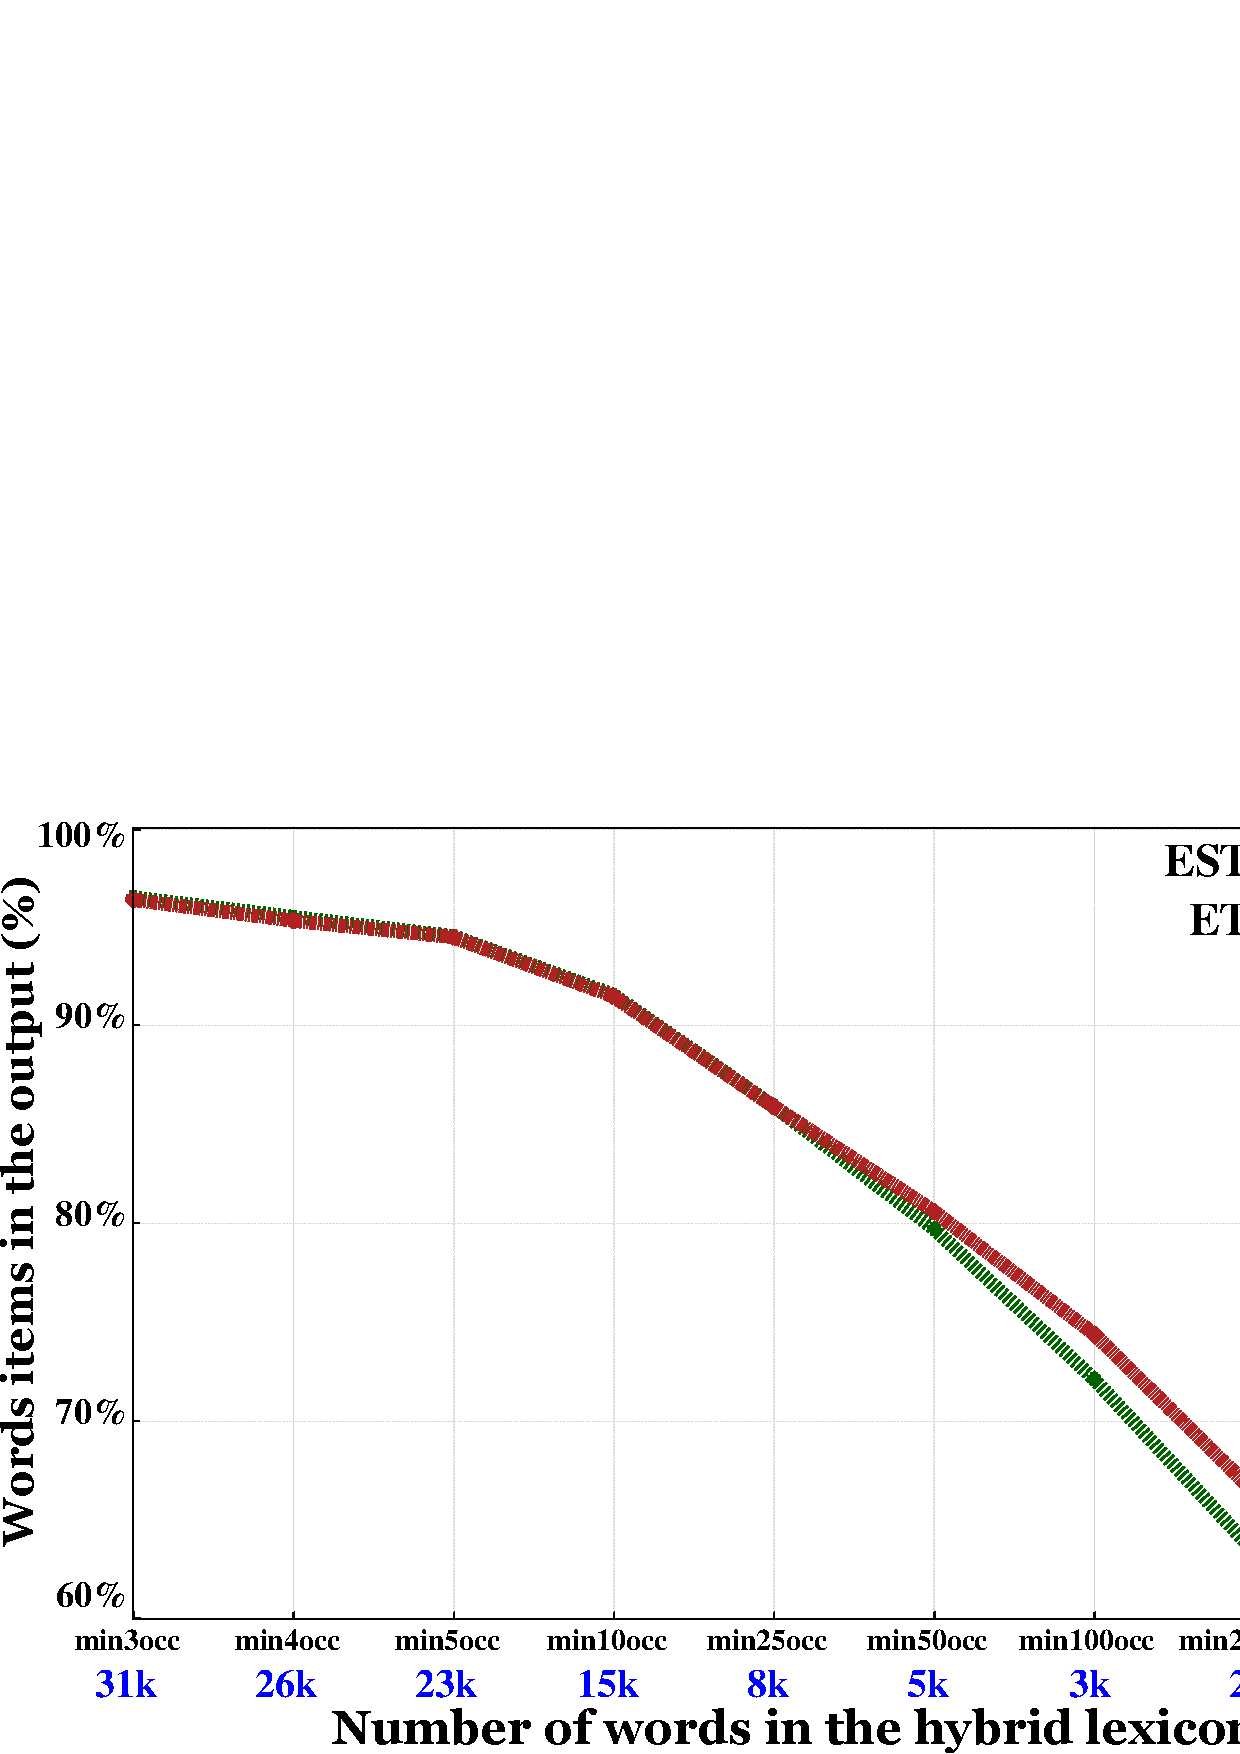
\includegraphics[scale=0.98]{Image/results/wordsInWS.pdf}
			\end{center}
		\end{column}
		\begin{column}{.29\textwidth}
			\hskip-3ex \textbf{\color{OrangeRed}$\ast$}  {\color{OrangeRed} Combien de mots}  \\
			\hskip-2.5ex ont été produits  \\
			\hskip-2.5ex par le décodeur ?
		\end{column}
		\end{columns}

		\vskip1ex
		{\color{blendedblue} \hrule }
		\vskip1ex

		\begin{columns}
		\begin{column}{.70\textwidth}
			\begin{center}
			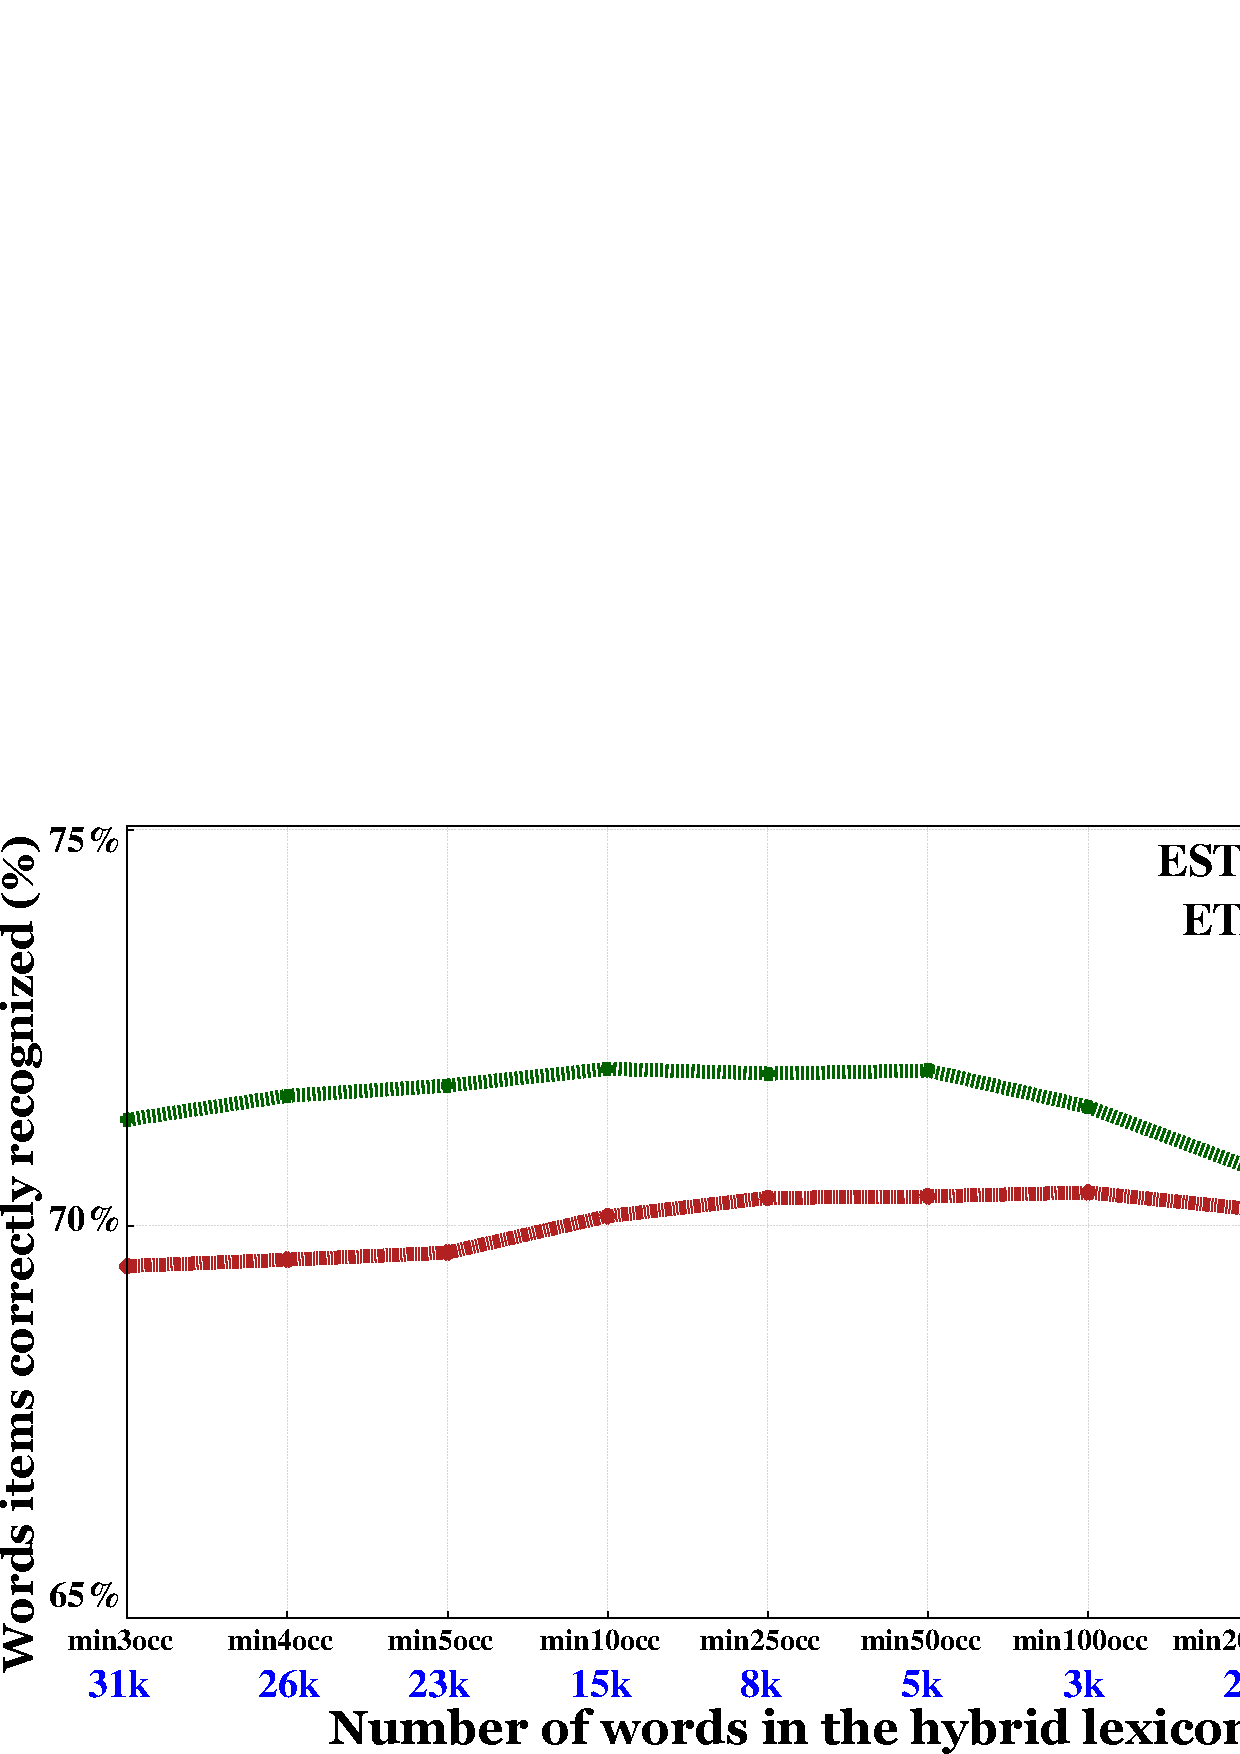
\includegraphics[scale=0.98]{Image/results/correctWordsInWS.pdf}
			\end{center}
		\end{column}
		\begin{column}{.29\textwidth}
			\hskip-3ex  \textbf{\color{OrangeRed}$\ast$} Parmi ces mots,  \\
			\hskip-2.5ex combien d'entre eux \\
			\hskip-2.5ex ont été {\color{OrangeRed} bien reconnus} ?
		\end{column}
		\end{columns}

		\vskip1ex
		{\color{blendedblue} \hrule }
		\vskip1ex

		\begin{columns}
		\begin{column}{.65\textwidth}
			\begin{center}
			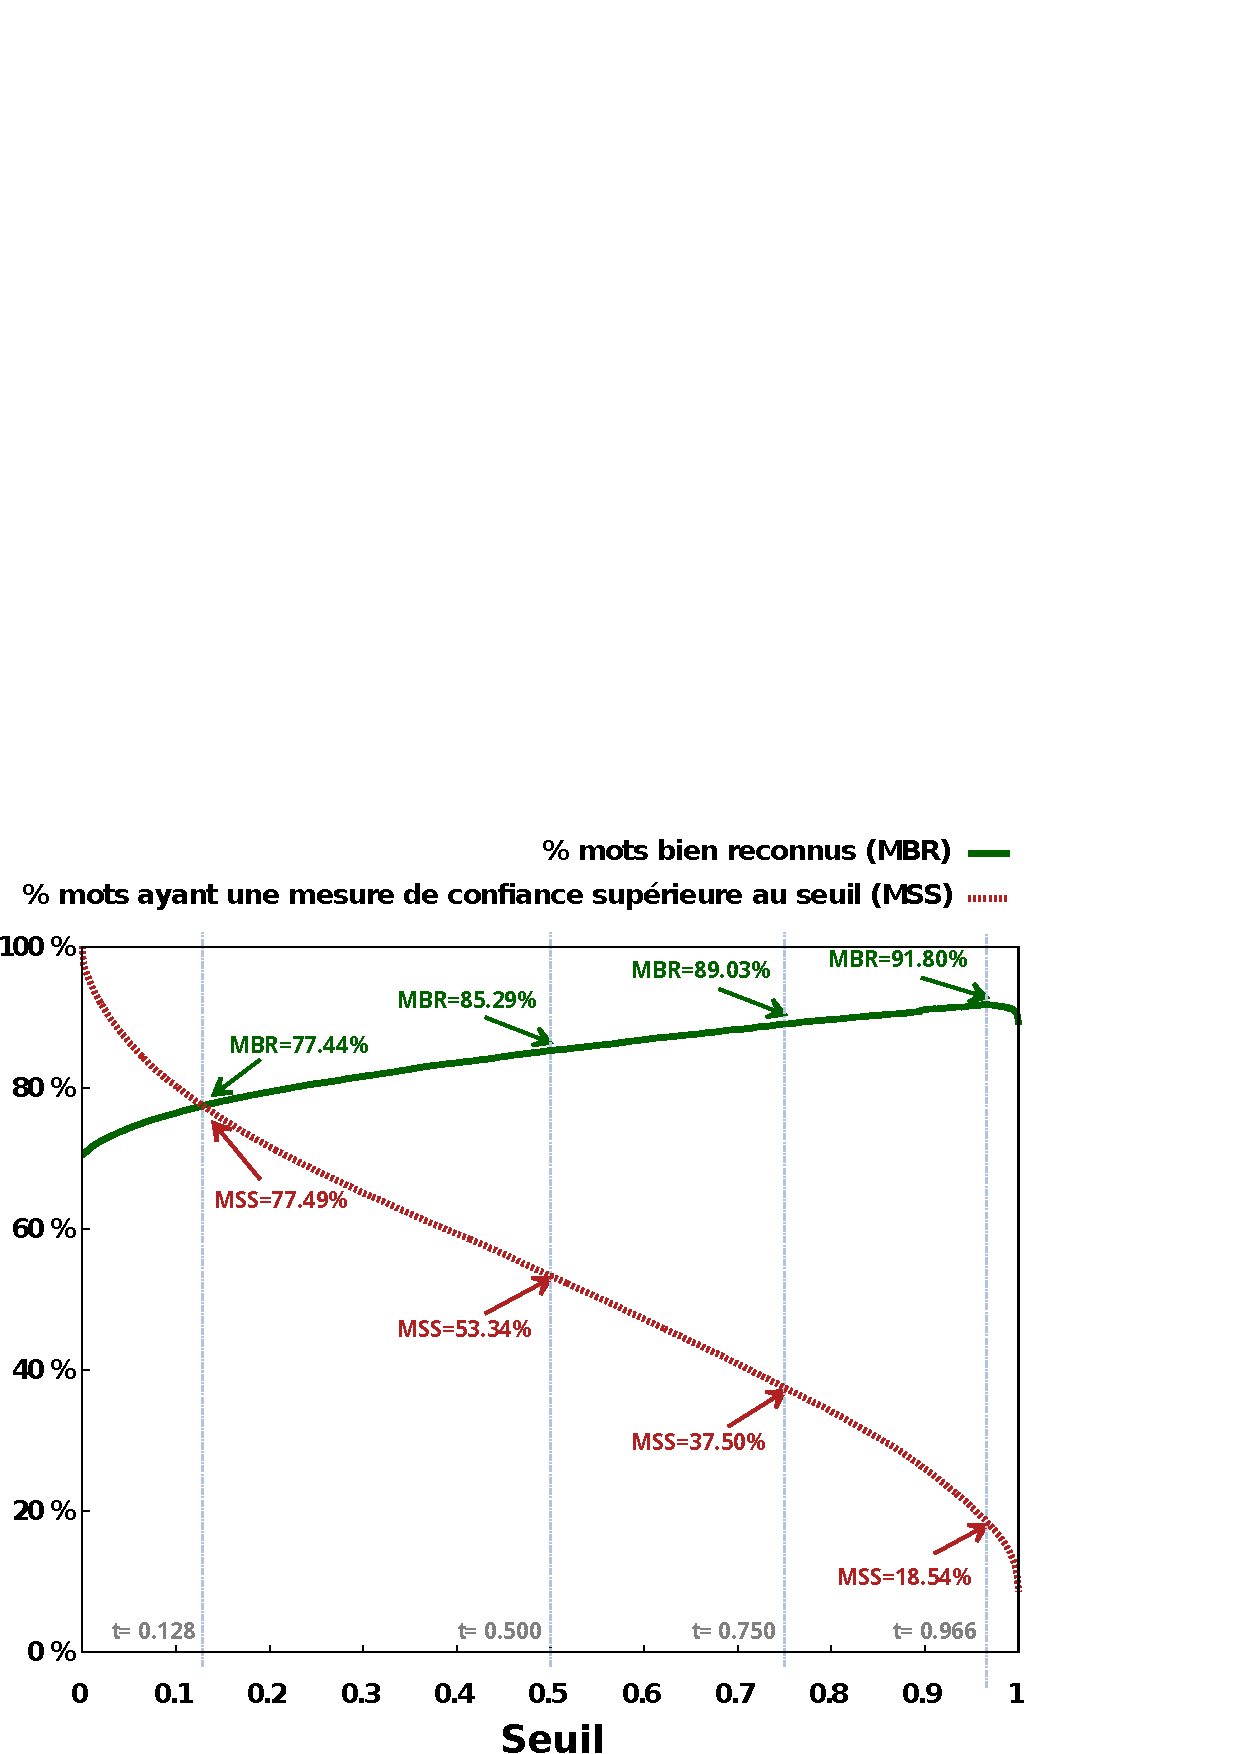
\includegraphics[scale=1.25]{Image/results/combined_min3occ_ETAPE.pdf}
			\end{center}
		\end{column}
		\begin{column}{.34\textwidth}
			\vskip9ex
			\hskip-3.3ex  {\color{OrangeRed}$\ast$} Les {\color{OrangeRed} mesures de confiance}  \\
			\hskip-2.8ex peuvent-elles identifier les  \\
			\hskip-2.8ex  {\color{OrangeRed} mots bien reconnus } ?
			\vskip9ex
			\hskip-2.8ex \textbf{\footnotesize $\rightarrow$ Corpus ETAPE, ML=min3occ}
		\end{column}
		\end{columns}

		\vskip1ex
		{\color{blendedblue} \hrule }
		\vskip1ex

		\begin{itemize}
		\item La contribution des {\color{OrangeRed} mesures de confiance sur les syllabes}
			\\ $\rightarrow$ pertinente seulement s’il existe une quantité relativement importante de syllabes dans le modèle de langage
		\end{itemize}
	\end{block}

	\vskip0.3ex
	\begin{block}{Conclusions}
		\begin{itemize}
			\item le modèle de langage hybride est un compromis efficace
			\item parmi les mots reconnus qui ont une mesure de confiance supérieure à 0.5, 85\% d'entre eux sont corrects
		\end{itemize}
	\end{block}

	\vskip0.3ex
	\begin{block}{Travaux futurs}
		\begin{itemize}
			\item étudier d'autres solutions pour mieux modéliser les syllabes à l'intérieur d'un modèle hybride
			\item analyser les mesures de confiance sur les syllabes
			\item analyser les segments correspondants aux mots hors vocabulaire
		\end{itemize}
	\end{block}
}


\end{minipage}
\end{beamercolorbox}
\end{column}
\end{columns}
\end{frame}
\end{document}

